\documentclass[a4paper]{report}
% Use swiss german letters
\usepackage[utf8]{inputenc}
% Language: english
\usepackage[english]{babel}
% Fancy Figures
\usepackage{graphicx}
% Use Times
\usepackage{mathptmx}
% Display the Bibliography in the TOC
\usepackage{tocbibind}
% Better lists
\usepackage{enumitem}
% Shaded Boxes
\usepackage[svgnames]{xcolor}
\usepackage{framed}
\usepackage{mdframed}
% Use biblatex
\usepackage[style=apa,backend=biber,citestyle=authoryear]{biblatex} 
% Define the bibliography file
\addbibresource{bibliography.bib}
% To let LaTeX handle "
\usepackage[autostyle, english = british]{csquotes}
\DeclareLanguageMapping{english}{english-apa}
% To have text wrap around pictures
\usepackage{wrapfig}
% Define Shaded box
\definecolor{grey}{HTML}{C5C5C5}
\definecolor{lightgrey}{HTML}{E6E6E6}
\definecolor{lightblue}{HTML}{F0F7FD}
\definecolor{greyblue}{HTML}{D0E3F0}
\definecolor{darkblue}{HTML}{3A87AD}
\newmdenv[topline=false,rightline=false,bottomline=false,linecolor=greyblue,linewidth=2pt,backgroundcolor=lightblue]{quotebox}
% Blindtext package
% TODO remove
\usepackage{blindtext}

% Titlepage
\newcommand*{\titleAP}{\begingroup % Create the command for including the title page in the document
	\centering
	\vspace*{\baselineskip} % Whitespace at the top of the page
	
	{\Large Thushjandan Ponnudurai} and {\Large Pascal Baumann}\\[0.167\textheight] % Author name
	
	{\Huge\bfseries Client-to-Client IPsec VPN with an OpenSSL CA in a mixed host environment}\\[\baselineskip]
	
	%TODO review subtitle
	{\Large \textit{Term paper NS FS2017}}\\
	\today
	
	\vspace*{3\baselineskip} % Whitespace at the bottom of the page
	\endgroup}

% Define the path were images are found
\graphicspath{{./img/}}

\begin{document}

\titleAP

\newpage

\begin{abstract}
	%TODO write abstract
	\blindtext
\end{abstract}

\tableofcontents

\newpage

\chapter{Theoretical part}
\label{ch:Theory}

\section{IP protocols}
\label{sec:IPprot}
The Internet Protocol (IP) is a set of rules governing how packets are transmitted over the Internet. IP is probably the common protocol in the internet and is one of the layer 3 protocols (network layer) in the OSI model. It implements two basic functions:
\begin{itemize}
	\item Addressing hosts
	\item Routing packets from a source host to a destination host over multiple IP networks
\end{itemize}
A packet is composed of an IP header and a payload. Source and destination IP addresses and other meta data are parts of the IP header and are required to deliver a packet. The payload includes data that is transported.

IPv4 is the first major version and is at the moment the dominant protocol version of the Internet. Due to a lack of IPv4 addresses the successor IPv6 was born. \parencite{NadeemUnuth2016}

\subsection{IPv4}
\label{ssec:IPv4}
Internet Protocol version 4 (IPv4) is specified in the IETF RFC 791 document \parencite{Postel} and has existed since 1980. To route a packet across the networks, every host in the network has a logical address, which is the IPv4 address. This IPv4 addressing system is based on a 32-bit logical address, which amounts to 4'294'967'296 unique addresses.

An example of an IPv4 address is "148.21.45.110". The address is written in dot decimal notation and it has four octets of 8-bits. The binary form of this address will be 10010100.00010101.00101101.01101110. \parencite{Babatunde2014}

At the moment there is an IPv4 address exhaustion problem. Since the 3th of February 2011 "Internet Corporation for Assigned Names and Numbers" (ICANN) doesn't have any free blocks of IPv4 addresses to distribute. Due this problem IPv6 was developed and everything will be migrated to IPv6 in the long-term. 
\subsection{IPv6}
\label{ssec:IPv6}
Internet Protocol version 6 (IPv6) is the successor of IPv4. It was specified in 1998. The growth of the Internet led to a need for alternatives. The problem is, that IPv4 cannot provide the needed number of logical addresses. For that reason IPv6 protocol was developed.\parencite[11]{Babatunde2014}

Several important areas were enhanced in the IPv6 protocol:
\begin{itemize}
	\item Expanded addressing
	\item Simplified header format
	\item Improved extension and option support
\end{itemize}
With the expanded address space the issue with the lack of addresses will be mitigated. Also the addressing architecture and the simplified header format are improving the routing efficiency. Fewer packets needs to be processed thanks to the simplified header format. 
Every IPv6 packet has a fixed header length of 40 octets. But any options can be appended in extension headers after the IPv6 main header. \parencite[106-107,123-124]{Loshin2004}

\subsubsection{IPv6 Addressing}
\label{sssec:ipv6:addressing}
There are three types of IPv6 addresses:
\begin{itemize}
	\item Unicast. A packet sent to an unicast address is delivered to the interface identified by that address.
	\item Multicast. A packet sent to a multicast address is delivered to all interfaces identified by that address. This address could be existing on different hosts.
	\item Anycast. A packet sent to a anycast address is delivered to one of the interfaces identified by that address. This address could be existing on different hosts.
\end{itemize}
The traditional IPv6 broadcast does not exist anymore, instead the functionality is provided by specific multicast addresses. To find a router for example, one can ping FF02::2, as any router interface will subscribe to this multicast address. \parencite[142-143]{Loshin2004}

The length of an IPv6 address is 128-bit. It is usually represented as 8 groups of up to 4 hexadecimal digits that are separated with colons. Each group stands for 16 bits.
\begin{quotebox}
	XXXX:XXXX:XXXX:XXXX:XXXX:XXXX:XXXX:XXXX
\end{quotebox}
Here is an example of an IPv6 address.
\begin{quotebox}
	2001:db8:1234:ABCD::10
\end{quotebox}
IPv6 addresses are usually divided into two equal 64-bit parts. The first 64-bit part identifies a network address and the last 64-bit part the host. \parencite[144-146]{Loshin2004}
 
\subsubsection{IPv6 Headers}
\label{sssec:ipv6:headers}
The length of an header in IPv6 is not variable like in IPv4. It has a fixed length of 40 bytes. An IPv4 header can be as short as 20 bytes and as long as 60 bytes due to the IP options. Routers usually process all the options in the IPv4 header, even if these options aren't relevant for the processing router. This leads to a degradation of the forwarding performance.  With the fixed header length in IPv6, packet handling is more efficient. \parencite[128]{Loshin2004}

In the figure \ref{fig:IPv4_IPv6_Header} the IPv6- and IPv4-header are presented. It shows that an IPv6 header is simpler that an IPv4 header. The reason is that many attributes were removed in IPv6.
\begin{figure}
	\centering
	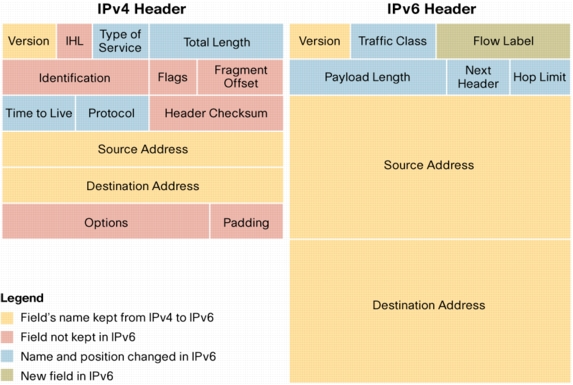
\includegraphics[width=0.8\linewidth]{ipv6_ipv4_headers}% no need to specify the file extension
	\caption {IPv4 and IPv6 Headers \parencite{cisco2006}}
	\label{fig:IPv4_IPv6_Header}
\end{figure}

The IP option field is very important for the IP protocol operation. The functionality of IP options were removed from the main header and implemented in the extension headers. Extension headers (EH) are a set of additional headers, which can be added as needed. So the routers will only process the main header and will process the extension headers only if it is required.

The figure~\ref{fig:IPv4_IPv6_ext_Header} explains how the extension headers are linked together in an IPv6 packet.
\begin{figure}
	\centering
	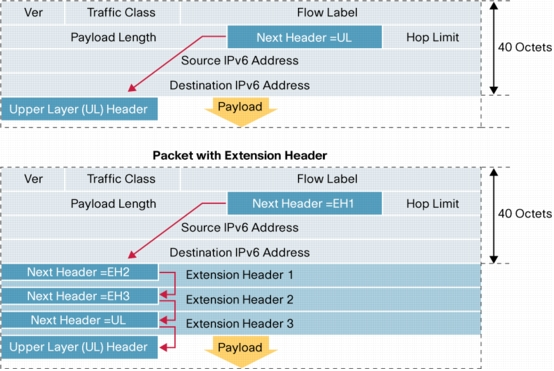
\includegraphics[width=0.8\linewidth]{ipv6_ipv4_ext_headers}% no need to specify the file extension
	\caption {IPv6 extension header chain \parencite{cisco2006}}
	\label{fig:IPv4_IPv6_ext_Header}
\end{figure}
The extension headers are defined in RFC 2460 and their are shown in the table~\ref{tab:extension_header_codes} along with the Next Header codes assigned to them. The recommended order, how the headers should be chained in a packet, is also defined in this RFC. \parencite[1-3]{cisco2006}
\begin{table}[]
	\centering
	\caption{Extension Headers and their recommended order in a packet}
	\label{tab:extension_header_codes}
	\begin{tabular}{lllll}
		\hline
		\textbf{Order}&  \textbf{Header Type}&  \textbf{Next Header Code}\\
		\hline
		1&  Basic IPv6 Header&  - \\
		2&  Hop-by-Hop Options
		Destination&  0 \\
		3&  Destination Options (with Routing Options)&  60 \\
		4&  Routing Header&  43 \\
		5&  Fragment Header&  44 \\
		6&  Authentication Header&  51 \\
		7&  Encapsulation Security Payload Header&  50 \\
		8&  Destination Options&  60 \\
		9&  Mobility Header&  135 \\
		&  No next header&  59 \\
		Upper layer&  TCP&  6 \\
		Upper layer&  UDP&  17 \\
		Upper layer&  ICMPv6&  58 \\
	\end{tabular}
\end{table}



\section{VPN protocol suites}
\label{sec:VPNs}

\subsection{SSL VPN}
\label{ssec:sslvpn}

SSL VPN is a transport layer VPN protocol. The encryption and connection establishment is done over the TLS protocol. TLS (Transport Layer Security) is the successor of the SSL protocol, and thus a part of the SSL protocol suite which is widely used in the web environment. Due to this widespread adaptation, implementing an SSL VPN in an enterprise environment is relatively trivial. As TLS is reliant on a reliable transport channel, its typically implemented over TCP. \parencite[6,96]{Dierks2008}

Therefore, SSL VPN (over TLS) suffers from the same problems that TCP has:

\begin{itemize}
	\item Not suited for time-critical applications, due to the time overhead
	\item Prone to SYN DoS attacks
\end{itemize}

These disadvantages led to the development of DTLS. The Datagram Transport Layer Security protocol has the same security guarantees as TLS but implements it over the datagram service. The fundamental problem faced when using the datagram service is the unreliability of packets (the order of packets, missing packets), which TLS can not handle as it depends on continuous sequence numbers to decrypt the received communication and a ensured transmission of all handshake messages. To work around these issues, DTLS bans stream ciphers (to avoid dependency on preceding packets), adds timers to detect missing handshake messages and adds explicit sequence messages. If a client or server receives a message too far ahead in the sequence, it caches it and uses it when all preceding messages are received. \parencite[5-15]{Rescorla2012}

Unrelated to which specific implementation of TLS is used (TLS over TCP, or DTLS), the application data is encrypted on the transport layer on the client and sent securely along the full path to the server.

\subsection{L2TP/PPTP}
\label{ssec:l2tppptp}
When discussing Layer Two Tunneling Protocol (L2TP) and Point-to-Point Tunneling Protocol (PPTP), one has to first understand the predecessor of them both: Point-to-Point Protocol (PPP).
The development of PPP arouse from the discontent with then de-facto standard for serial links SLIP. The role of SLIP was to bridge the gap between IP and serial links, which it does, but not more. The wish for a general purpose protocol, able to encapsulate multiple different higher layer protocols and with support for different physical link layer configurations. PPP was based on the ISO standards protocol HDLC and adapted the framing structure and some operation concepts from it.  \parencite{Kozierok2005}

PPTP in turn describes a protocol for tunneling PPP traffic over an IP network. It does not change the implementation or modify the encapsulated PPP traffic. As its just a vehicle for transporting PPP traffice, PPTP does not offer authentication nor encryption, as this is handled by the PPP protocol itself (with PAP/CHAP and ECP respectively). The beauty of PPTP is, that it can be encapsulated in the IP payload, so that only the two endpoints talking to each other have to implement it. PPTP has a control channel which is initiated over TCP and a modified GRE protocol for the tunnel itself. \parencite{Hamzeh1999}

L2TP as a protocol enables to route PPP over a layer two network. Before L2TP a PPP session had to be terminated at the layer two endpoint. L2TP enables that the PPP traffic is passed on to a Network Access Server (NAS) and divorces the PPP and layer two traffic. The L2TP tunnel splits its traffic into a data and control channel. The data traffic is encapsulated by a L2TP header and then passed over an unreliable channel (UDP, Frame Relay, etc.), whereas the control traffic is passed over a reliable channel. Before PPP traffic is passed over the tunnel, an L2TP session has to be established over the control channel. Authentication is over a CHAP-like mechanism and necessitates a single pre-shared secret. \parencite{Townsley1999}



\subsection{IPsec}
\label{ssec:IPsec}
IPsec is a widely used tunneling protocol suite. As it is a suite, there are many different interlocking parts and many considerations to be made when deploying IPsec. But as stated in \cite{Bellovin2009}: \textquotedblleft These [parts] can be used to provide confidentiality, integrity, and replay protection;\textquotedblright.
In this paragraph we want to introduce some key concepts for IPsec which will be discussed in more detail in section \ref{sec:IPsec}.
The first question one has to ask oneself is, which security protocol to use - Authentication Header (AH) or Encapsulating Security Payload (ESP), or both simultaneously. 

The AH hashes the whole original IP packet (in tunnel mode) or just the higher-layer protocol header and data (in transport mode). Upon receival, the receiving party can verify these hashes and recognize tampering; this makes the AH security protocol irreconcilable with the NAT method. \parencite[2-11]{Kent2005AH}

Analogous to the AH protocol, ESP can work both in transport and tunnel mode. Simultaneously, in transport mode, the ESP header is inserted after the original IP header and encrypts the higher-level protocol header and data, whereas in tunnel mode, the ESP protocol encapsulates the whole IP packet and generates a new IP header. \parencite[18-20]{Kent2005ESP}

The next consideration concerns the key management. Although manual key management can be used, it's generally not advised and disables the replay detection mechanism.The most widely used key management is the Internet Key Exchange (IKE), which is available in its original form (IKEv1) and in a new, simpler version (IKEv2). In network environment where mainly Microsoft systems are used, the usage of Kerberised Internet Negotiation of Keys (KINK) is available, as this depends on the Kerberos system. \parencite[4-5]{Bellovin2009}

\section{ISAKMP}
\label{sec:ISAKMP}

\subsection{Algorithms \& DHs}
\label{ssec:AlgoDH}
Data confidentiality is the key requirement for any VPN. The confidentiality of the data is provided by the encryption algorithm. That's why it is very important to choose the optimal encryption algorithm. \parencite{Snader2006}

Every encryption algorithm can be theoretically broken with given enough computing resources. With a brute-force attack every combination of a key will be try out. "For a 128-bit key, there are $2^{128}$ combinations to attempt, which requires extensive computing resources." according to \cite{HigashiMichael2013}. 
The data confidentiality can be only ensured with the correct key length (ex. for AES more than 256-bits or for RSA more than 2048-bits). 

It is possible to decrypt a message without knowing the key with enough computing resources and time. But the decrypted information will be too old and not more relevant for the attacker. 
That's why it is very important to choose strong and long passwords/keys to make the decryption difficult for the attacker.\parencite{HigashiMichael2013}

There are two categories of cryptography algorithms: Symmetric and Asymmetric

\subsubsection{Symmetric}
\label{sssec:symmetric}
Sender and receiver are using the same secret key to encrypt and to decrypt the messages. The main problem with these categories of algorithms is finding a way to distribute the key without anyone else finding it.

Some symmetrical algorithms:
\begin{itemize}
	\item AES (128, 192 or 256 bit)
	\item DES (56-bit)
	\item Triple-DES or 3DES (3x 56-bit = 168-bit).
	\item Blowfish (128, 192 or 256 bit)
	\item CAST (128-bit)
	\item Camellia (128, 192 or 256 bit)
\end{itemize}
AES-256 is commonly used in VPNs. DES is not secure anymore, because a DES key can be cracked in less than 24 hours. \parencite{Bollapragada2005}

\subsubsection{Asymmetric}
\label{sssec:asymmetric}
Asymmetrical algorithms, also known as public key algorithm, use separate keys for encryption and decryption. The public key is used for the encryption and can be made public. The private key is used for decryption and must be kept secret. The public key and private key are mathematically related, but it is not possible to find out the private key from the public key. 

The key advantage of an asymmetrical algorithm is the ease of distribution of the encryption/decryption key. Only the private key must be kept securely. The public key can be distributed to anyone.
A drawback for asymmetric algorithms is, that they are typically slower than symmetrical algorithms. They involves exponential operations, which needs more CPU cycles. Asymmetric algorithms are often used to secure key exchanges rather than used for bulk data encryption.

RSA, DSA and Elliptic Curve Cryptography (ECC) are some asymmetrical algorithms. \parencite{Bollapragada2005}

Figure \ref{fig:asym_alg} shows how typically a public key encryption works. The process starts with negotiating a public key algorithm and ends with the decryption of Alice's message.
\begin{figure}[htb]
	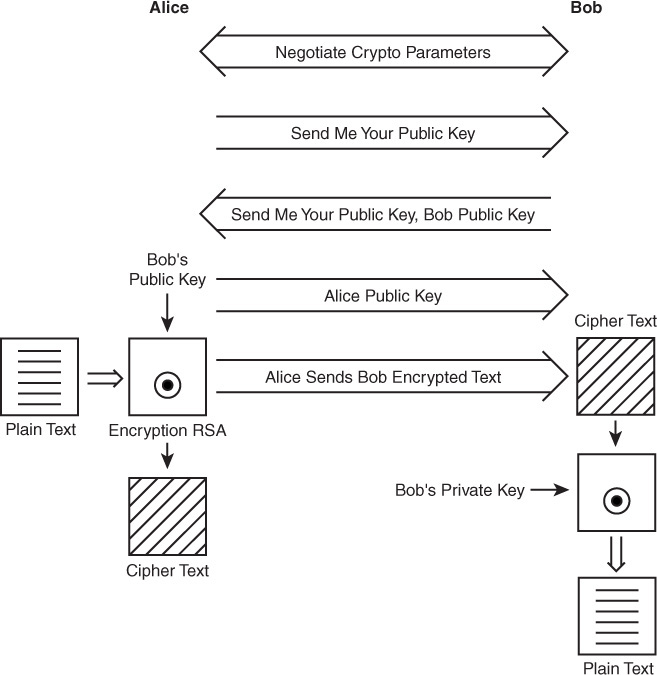
\includegraphics[width=\linewidth]{asym_alg.jpg}
	\caption{Public Key Encryption process}
	\label{fig:asym_alg}
\end{figure}

\subsubsection{Diffie-Hellman (DH)}
\label{sssec:diffie-hellman}
With Diffie-Hellman algorithm (DH) two devices can establish a shared secret over an unsecure network. It was published by Whitfield Diffie and Martin Hellman in 1976. Related to VPN, it is used in IKE Phase 1 and 2 for key exchange. 

Diffie Hellman group are used to specify the strength of the session key used in the DH key exchange process. Higher DH group numbers are more secure, but require additional processing resources to compute the session key. \parencite{JajishThomas}
\begin{itemize}
	\item \textbf{DH group 1}: 768-bit modulus
	\item \textbf{DH group 2}: 1024-bit modulus
	\item \textbf{DH group 5}: 1536-bit modulus
	\item \textbf{DH group 14}: 2048-bit modulus
	\item \textbf{DH group 15}: 3072-bit modulus
	\item \textbf{DH group 19}: 256-bit elliptic curve group
	\item \textbf{DH group 20}: 384-bit elliptic curve group
	\item \textbf{DH group 21}: 521-bit elliptic curve group
	\item \textbf{DH group 24}: 2048-bit modulus with 256 bit Prime Order subgroup
\end{itemize}

At the moment it is strongly recommended to use at least \textbf{DH group 14}. If an encryption or authentication algorithm with a 256-bit key or higher is used, then it is recommended to use DH group 21 or 24. \parencite{StrongSwan}

\subsubsection{Hashing Algorithm}
\label{sssec:hashing_algo}
"Hash algorithms are also called \textit{digital fingerprinting algorithms}. They are mathematically irreversible functions that provide a fixed-size hash based on various inputs. Irreversibility and collision resistance are necessary attributes for successful hash functions." \parencite{Kampanakis2015}
Message-Digest-Algorithm 5 (MD5), Secure Hash Algorithm 1 (SHA-1) or SHA-2 are some examples of hashing algorithms. MD5 and SHA-1 are \textbf{insecure} and should not be used anymore. 

A Keyed-Hash Message Authentication Code (HMAC) is a type of message authentication codes (MAC) that uses a secret key and a cryptographic hash function. It is used for 
\textbf{integrity verification}.

There are existing several HMAC algorithms with various key length. Some of them are listed in the following list:
\begin{itemize}
	\item HMAC-SHA-2 with 512-, 384-, 256-, 192-, 128-bits key length
	\item AES-GMAC with 256-, 192- or 128-bits key lengths (Same as AES-GCM, but without encryption)
	\item SHA-1 HMAC
	\item MD5 HMAC
\end{itemize}

\subsection{IKE Phase 1}
\label{ssec:Phase1}
"Phase 1 of an AutoKey Internet Key Exchange (IKE) tunnel negotiation consists of the exchange of proposals for how to authenticate and secure the channel." \parencite{JuniperNetworks2016} The result of this phase is the establishment of an ISAKMP/IKE security association (SA). Mandatory parameters for negotiating an IKE SA are the encryption algorithm, hash algorithm, authentication mode (preshared-key or RSA/DSA certificates) and Diffie-Hellman (DH) group.

IKE Phase 1 offers two modes: Main mode and aggressive mode.
\subsubsection{Main mode}
\label{sssec:Phase1:mainMode}
The initiator and recipient send three two-way exchanges, with a total of six messages:
\begin{itemize}
	\item First exchange. Proposes and accepts the encryption and authentication algorithms.
	\item Second exchange. Executes a DH exchange and exchanges keying material. After this stage  the remaining messages (Third exchange) are encrypted.
	\item Third exchange.  Verifies the other side's identity.
\end{itemize}

\subsubsection{Aggressive Mode}
\label{sssec:Phase1:aggressiveMode}
The initiator and recipient have only two exchanges, with a total of three messages:
\begin{itemize}
	\item First message. Almost everything will be sent: SA proposes, DH public key, keying material and also its own identity.
	\item Second message. The receiver authenticates the initiator and sends everything back that is needed to complete the exchange.
	\item Third message. The initiator authenticates the recipient and confirms the exchange.
\end{itemize}
Aggressive mode is faster than the main mode, but it does not provide the identity protection! The reason therefore is, that both sides exchanges their identities before a secure channel exists. \parencite{JuniperNetworks2016}

\subsection{IKE Phase 2}
\label{ssec:Phase2}
After a secure IKE tunnel is established in the first phase, there is a second round of exchanging key information and building security associations (SA). "A security association (SA) is a set of policy and key(s) used to protect information. The ISAKMP SA is the shared policy and key(s) used by the negotiating peers in this protocol to protect their communication." \parencite{Harkins1998} After obtaining possibly multiple SAs, the IPsec tunnel is finally formed and the peers exchange information encrypted with the SAs. In the so called quick mode, the peers negotiate a common IPsec policy and secret keying material, which in turn lead to the IPsec SAs. If Perfect Forward Secrecy (PFS) is demanded, a new Diffie-Helman key exchange is performed through the secure ISAKMP tunnel. This ensures the keys from phase one be completely unrelated to the keys from phase two. The drawback of this is the additional computations needed to complete the DH key exchange.

\section{IPv6 with IPsec}
\label{sec:IPv6IPsec}

\chapter[Practical part\\Client-to-Client IPsec VPN with an OpenSSL CA in a mixed host environment]{Practical part\\\large{Client-to-Client IPsec VPN with an OpenSSL CA in a mixed host environment}}
\label{ch:Practical}

\section{Description of the experiment}
\label{sec:ExpDesc}

In our experiment we will connect to host machines in separate IPv6 networks over two routers, as shown in figure \ref{fig:exp_layout}. On our connecting network, we will have a certificate authority for our local domain nl.ch and a machine running Wireshark. The man-in-the-middle machine will be our control, if the transmission between the two hosts is indeed encrypted or not. For that we will prepare a script, that periodically sends a String via ncat to the receiver.

\subsection{Experiment layout}
\label{ssec:ExpLayout}

\begin{figure}[htb]
	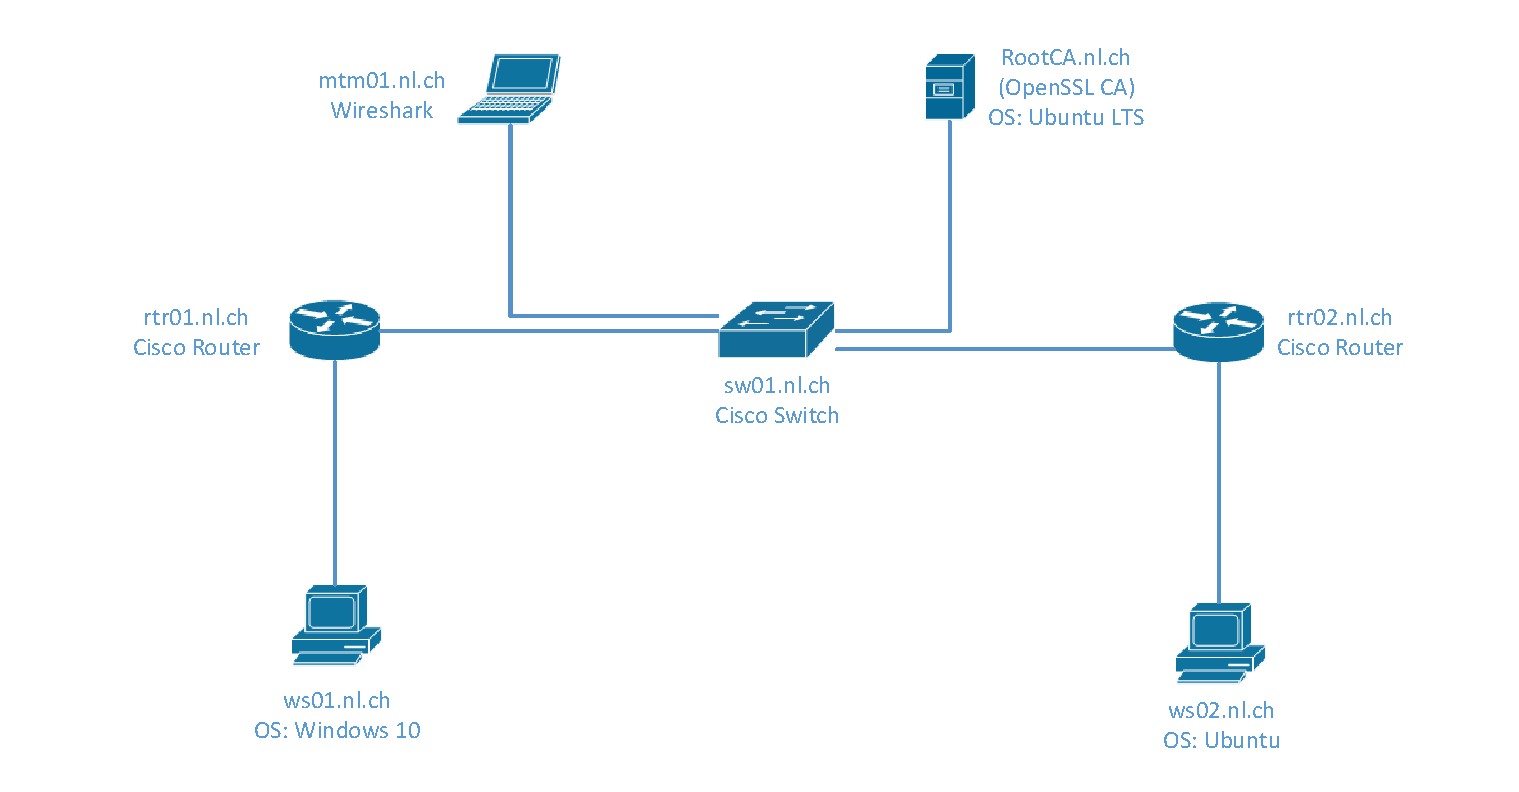
\includegraphics[keepaspectratio, width = \linewidth]{experiment_layout}
	\caption{The setup which will be used in our experiment}
	\label{fig:exp_layout}
\end{figure}

\subsection{Network addressing concept}
\subsubsection{client network 01}
\begin{tabular}{|c|c|}
	\hline 
	\textbf{device} & \textbf{IPv6 address} \\ 
	\hline 
	rtr01 & FD00:DEAD:CAFE:1::1/64 \\ 
	\hline 
	ws01 & FD00:DEAD:CAFE:1::2/64 \\ 
	\hline 
\end{tabular} 

\subsubsection{client network 02}
\begin{tabular}{|c|c|}
	\hline 
	\textbf{device} & \textbf{IPv6 address} \\ 
	\hline 
	rtr02 & FD00:DEAD:CAFE:2::1/64 \\ 
	\hline 
	ws02 & FD00:DEAD:CAFE:2::2/64 \\ 
	\hline 
\end{tabular} 

\subsubsection{transport network}
\begin{tabular}{|c|c|}
	\hline 
	\textbf{device} & \textbf{IPv6 address} \\ 
	\hline 
	rtr01 & FD00:DEAD:CAFE:3::1/64 \\ 
	\hline 
	rtr02 & FD00:DEAD:CAFE:3::2/64 \\ 
	\hline 
	rootCA & FD00:DEAD:CAFE:3::A/64 \\ 
	\hline 
\end{tabular} 

\section{Expected results}
\label{sec:ExpectedResult}
We expect that we will see the various phases on both clients. We expect to have problems with the algorithms used, specifically we expect that the Windows client will have predefined SAs which we won't be able to change. Therefore we will have to amend our Ubuntu client to match the requirements of his peer.

\begin{figure}[htb]
	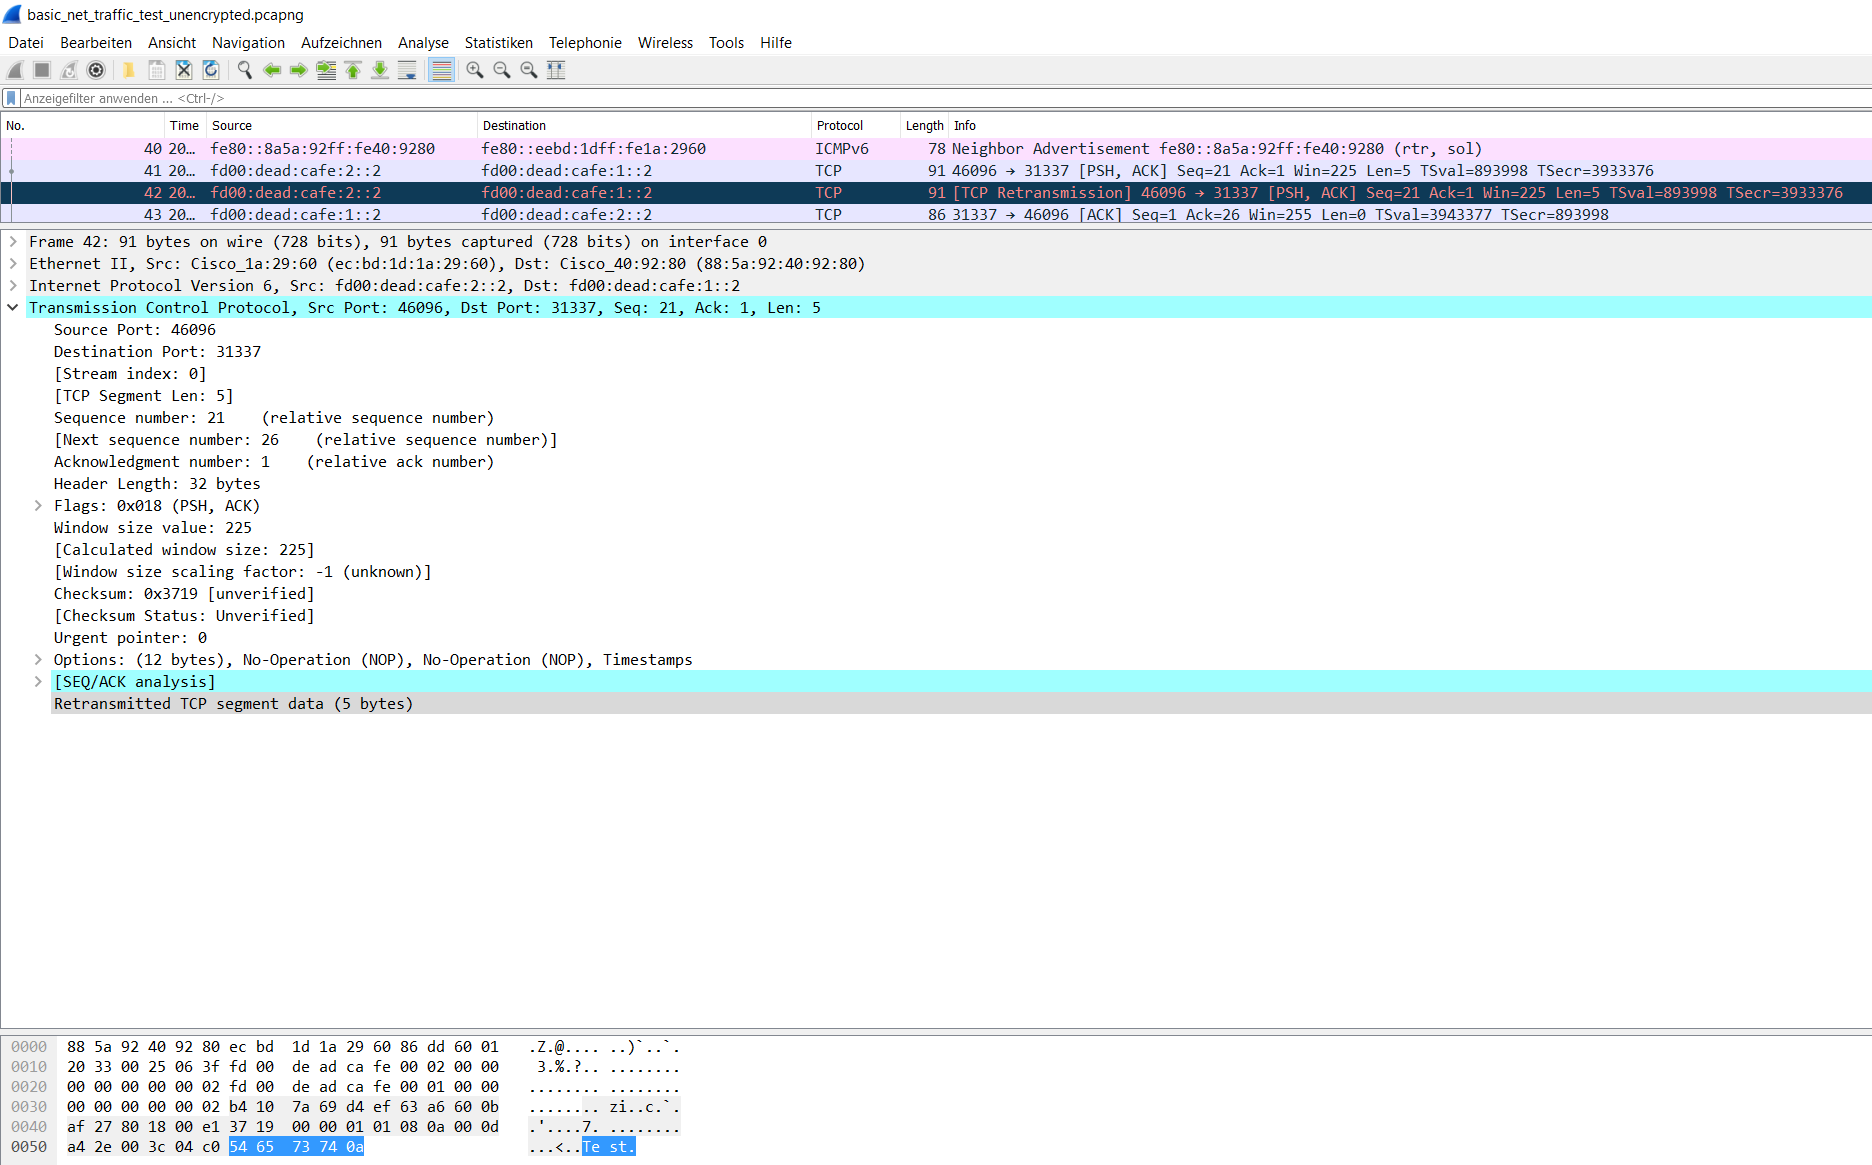
\includegraphics[width=\linewidth]{Testscript_unencrypted.png}
	\caption{TCP communication between hosts, captured in Wireshark}
	\label{fig:TestUnencrypted}
\end{figure}


\section{Experiment execution}
\label{sec:ExpExec}
We used two Cisco %TODO insert model of router
where we connected the Cisco %TODO insert model of switch
to the GigabitEthernet0/0 interfaces. Our clients where connected to the GigabitEthernet0/1 interfaces respectively. The setup of the whole network was done without a problem. After testing our connections (to the router and our peer) and recognising that the Windows Firewall was blocking our connection attempts, we tested the viability of our test script. After installing the necessary components (nmap and Zenmap) the script was sending our test string without a problem, and we were able to catch this traffic with our MITM machine as can be seen in figure \ref{fig:TestUnencrypted}. 

The configuration of the openSSL root CA server was done with the tutorial of %TODO insert link here
After the configuration of the certificate authority, we generated two certificates for our hosts. Due to problems exporting these certificates and time constraints, we advanced to building the IPsec tunnel. As we did not have valid certificates ready yet, we opted to use a preshared key for our IPsec tunnel.

Contrary to our expectations, the configuration of the IPsec tunnel on our Windows 10 client (further referred as ws01) was very simple and comprehensive. In ws01 we had to configure the tunnel rules on the firewall itself, and under the options which kind of algorithms will be used for the establishment for the tunnel.
On the Ubuntu client (hereafter referred to as ws02) we noticed, that we had not yet installed an IPsec VPN client. After a short research we concluded, that StrongSwan best suits our need.

\section{Experiment results}
\label{sec:ExpRes}

\section{Conclusion}
\label{sec:Conc}

\newpage

\printbibliography

\end{document}          
